\documentclass[11pt]{article}
\usepackage[scaled=0.92]{helvet}
\usepackage{geometry}
\geometry{letterpaper,tmargin=1in,bmargin=1in,lmargin=1in,rmargin=1in}
\usepackage[parfill]{parskip} % Activate to begin paragraphs with an empty line rather than an indent %\usepackage{graphicx}
\usepackage{amsmath,amssymb, mathrsfs,  mathtools, dsfont}
\usepackage{tabularx}
\usepackage{tikz-cd}
\usepackage[font=footnotesize,labelfont=bf]{caption}
\usepackage{graphicx}
\usepackage{xcolor}
%\usepackage[linkbordercolor ={1 1 1} ]{hyperref}
%\usepackage[sf]{titlesec}
\usepackage{natbib}
\usepackage{../../Tianpei_Report}

%\usepackage{appendix}
%\usepackage{algorithm}
%\usepackage{algorithmic}

%\renewcommand{\algorithmicrequire}{\textbf{Input:}}
%\renewcommand{\algorithmicensure}{\textbf{Output:}}



\begin{document}
\title{Lecture 9: Integral Curves and Flows}
\author{ Tianpei Xie}
\date{Oct. 16th., 2022}
\maketitle
\tableofcontents
\newpage
\section{Integral Curves}
\begin{itemize}
\item  Suppose $M$ is a smooth manifold with or without boundary. If $\gamma: J \rightarrow M$ is a smooth curve, then for each $t \in J$, the velocity vector $\gamma'(t)$ is a vector in $T_{\gamma(t)}M$.

\begin{figure}
\begin{minipage}[htb]{1\linewidth}
  \centering
  \centerline{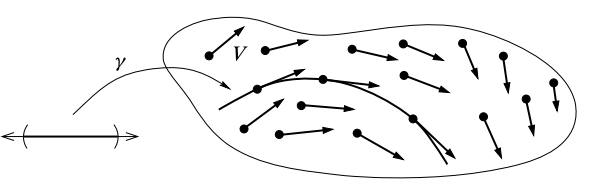
\includegraphics[scale = 0.5]{integral_curves.png}}
\end{minipage}
\caption{\footnotesize{\textbf{An integral curve of a vector field \citep{lee2003introduction}}}}
\label{fig: integral_curves}
\end{figure}

\item \begin{definition}
 Suppose $M$ is a smooth manifold with or without boundary and $V$ is a \emph{vector field} on $M$.  An \underline{\emph{\textbf{integral curve}}} of $V$ is a \emph{differentiable curve} $\gamma: J \rightarrow M$ whose \emph{\textbf{velocity}} at each point is equal to the \emph{\textbf{value of $V$}} at that point:
 \begin{align*}
 \gamma'(t) &= V_{\gamma(t)}, \quad \forall t\in J.
 \end{align*} (See Fig. \ref{fig: integral_curves}) If $0 \in J$, the point $\gamma(0)$ is called \emph{\textbf{the starting point of $\gamma$}}.
\end{definition}




\item \begin{example} (\textbf{Integral Curves})
\begin{enumerate}
\item Let $(x, y)$ be \emph{standard coordinates} on $\bR^2$, and let $V = \partdiff{}{x}$ be the \emph{\textbf{first coordinate vector field}}. It is easy to check that the integral curves of $V$ are precisely \emph{\textbf{the straight lines}} parallel to the $x$-axis, with parametrizations of the form $\gamma(t) = (a + t, b)$ for constants $a$ and $b$. (Fig, \ref{fig: vector_fields_integral_curve} (a))

\item Let $W = x \partdiff{}{y} - y \partdiff{}{x}$ on $\bR^2$ (Fig. \ref{fig: vector_fields_integral_curve}(b)). If $\gamma: \bR \rightarrow \bR^2$ is a smooth curve, written in standard coordinates as $\gamma(t) = (x(t), y(t))$,  then the condition $\gamma'(t) = W_{\gamma(t)}$ for $\gamma$ to be an integral curve translates to
\begin{align*}
x'(t) \partdiff{}{x}\Bigr|_{\gamma(t)} + y'(t) \partdiff{}{y}\Bigr|_{\gamma(t)} &=  x(t) \partdiff{}{y}\Bigr|_{\gamma(t)} - y(t) \partdiff{}{x}\Bigr|_{\gamma(t)}.
\end{align*} Comparing the components of these vectors, we see that this is equivalent to the system of ordinary differential equations
\begin{align*}
x'(t) &= - y(t) \\
y'(t) &=  x(t).
\end{align*} These equations have the solutions:
\begin{align*}
x(t)&= a\cos(t) -  b\sin(t) \\
y(t)&= a\sin(t) + b\cos(t)
\end{align*} for arbitrary constants $a$ and $b$, and thus each curve of the form $\gamma(t) = (a\cos(t) - b \sin(t), a \sin(t) + b \cos(t))$ is an integral curve of $W$. 
\end{enumerate}
\end{example}

\item \begin{remark}
Finding integral curves boils down to solving \emph{a system of ordinary differential equations} in a smooth chart.  Suppose $\gamma: J \rightarrow M$ is a smooth curve and $V$ is a smooth vector field on $M$. On a smooth coordinate domain $U \subseteq M$, we can write $\gamma$ in local coordinates as $\gamma(t) = (\gamma^{1}(t), \ldots, \gamma^{n}(t))$. Then the condition $\gamma'(t) =  V_{\gamma(t)}$ for to be an integral curve of $V$ can be written
\begin{align}
\dot{\gamma}^{i}\partdiff{}{x^{i}}\Bigr|_{\gamma(t)} &= V^{i}(\gamma(t))\partdiff{}{x^{i}}\Bigr|_{\gamma(t)}, \label{eqn: integral_curve_differential_equations_1}
\end{align} which reduces to the following \emph{\textbf{autonomous system of ordinary differential equations (ODEs)}}:
\begin{align}
\dot{\gamma}^{i}(t) &= V^{i}(\gamma^{1}(t), \ldots, \gamma^{n}(t)), \qquad i=1,\ldots, n.
\end{align}
\end{remark}

\begin{figure}
\begin{minipage}[htb]{1\linewidth}
  \centering
  \centerline{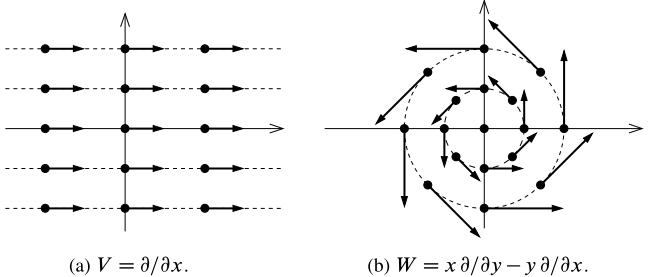
\includegraphics[scale = 0.5]{vector_fields_integral_curve.png}}
\end{minipage}
\caption{\footnotesize{\textbf{Vector fields and their integral curves \citep{lee2003introduction}}}}
\label{fig: vector_fields_integral_curve}
\end{figure}

\item The fundamental fact about such systems is \textbf{the \emph{existence}, \emph{uniqueness}, and \emph{smoothness theorem}} from ODE theory \citep{amann2011ordinary, hirsch2012differential}.
\begin{proposition}
Let $V$ be a smooth vector field on a smooth manifold $M$. For each point $p \in M$, there exist $\epsilon > 0$ and a smooth curve $\gamma: (-\epsilon, \epsilon) \rightarrow M$ that is an integral curve of $V$ starting at $p$.
\end{proposition}

\item The next two lemmas show how affine reparametrizations affect integral curves.
\begin{lemma} (\textbf{Rescaling Lemma}). \citep{lee2003introduction}\\
Let $V$ be a smooth vector field on a smooth manifold $M$, let $J \subseteq \bR$ be an interval, and let $\gamma: J \rightarrow M$ be an integral curve of $V$. For any $a \in \bR$, the curve $\widetilde{\gamma}: \widetilde{J} \rightarrow M$ defined by $\widetilde{\gamma}(t) =  \gamma(at)$ is an integral curve of the vector field $aV$, where $\widetilde{J} = \set{t: at \in J}$. 
\end{lemma}

\item \begin{lemma} (\textbf{Translation Lemma}).  \citep{lee2003introduction}\\
Let $V, M, J$, and $\gamma$ be as in the preceding lemma. For any $b \in \bR$, the curve $\widehat{\gamma}:  \widehat{J} \rightarrow M$ defined by $\widehat{\gamma}(t) =  \gamma(t + b)$ is also an integral curve of $V$, where $ \widehat{J} = \set{t: t + b \in J}$.
\end{lemma}

\item \begin{proposition} (\textbf{Naturality of Integral Curves}).  \citep{lee2003introduction}\\
Suppose $M$ and $N$ are smooth manifolds and $F: M \rightarrow N$ is a smooth map. Then $X \in \mathfrak{X}(M)$ and $Y \in \mathfrak{X}(N)$ are $F$-related \textbf{if and only if} $F$ takes integral curves of $X$ to integral curves of $Y$, meaning that for each integral curve $\gamma$ of $X$,  $F \circ \gamma$ is an integral curve of $Y$.
\end{proposition}
\begin{proof}
Suppose first that $X$ and $Y$ are $F$-related, and $\gamma:  J \rightarrow M$ is an integral curve of $X$. If we define $\sigma: J \rightarrow N$ by $\sigma = F \circ \gamma$ (see Fig. \ref{fig: Flows_F_related_vector_fields}), then
\begin{align*}
\sigma'(t) &= (F \circ \gamma)'(t) =  dF_{\gamma(t)}(\gamma'(t)) = dF_{\gamma(t)}(X_{\gamma(t)}) = Y_{F(\gamma(t))} = Y_{\sigma(t)},
\end{align*} so $\sigma$ is an integral curve of $Y$.

Conversely, suppose $F$ takes integral curves of $X$ to integral curves of $Y$. Given $p \in M$, let  $\gamma: (-\epsilon, \epsilon) \rightarrow M$ be an integral curve of $X$ starting at $p$. Since $F \circ \gamma$ is an integral curve of $Y$ starting at $F(p)$,  we have
\begin{align*}
Y_{F(p)} = (F \circ \gamma)'(0) = dF_{p}(\gamma'(0)) = dF_{p}(X _{p})
\end{align*} which shows that $X$ and $Y$ are $F$-related. \qed
\end{proof}
\end{itemize}

\begin{figure}
\begin{minipage}[htb]{1\linewidth}
  \centering
  \centerline{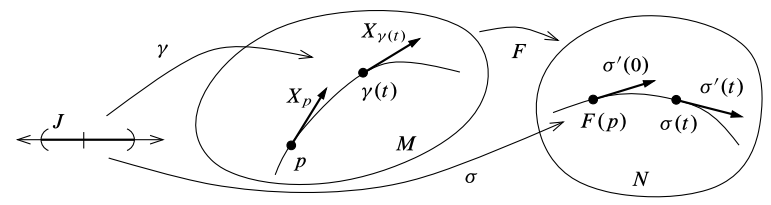
\includegraphics[scale = 0.45]{Flows_F_related_vector_fields.png}}
\end{minipage}
\caption{\footnotesize{\textbf{Flows for $F$-related vector fields \citep{lee2003introduction}}}}
\label{fig: Flows_F_related_vector_fields}
\end{figure}
\section{Flows}
\subsection{Global Flows}
\begin{itemize}
\item \begin{definition}
A \underline{\emph{\textbf{global flow on $M$}}} (also called \textbf{\emph{a one-parameter group action}}) is defined as a \emph{\textbf{continuous left $\bR$-action on $M$}}; that is, a \emph{continuous map} $\theta: \bR \times M \rightarrow M$ satisfying the following properties for all $s, t \in \bR$ and $p \in M$:
\begin{align}
\theta(t, \theta(s, p)) = \theta(t+s, p), \quad \theta(0, p) = p \label{eqn: global_flow}
\end{align}
\end{definition}

\item For a global flow $\theta$ on $M$, we define two collections of maps as follows:
\begin{itemize}
\item \begin{definition}
For each $t\in \bR$, \textbf{\emph{define}} a continuous map $\theta_t: M \rightarrow M$ by 
\begin{align*}
\theta_t(p) &= \theta(t, p). 
\end{align*} The defining properties in \eqref{eqn: global_flow} are equivalent to \emph{\textbf{the group laws}}:
\begin{align}
\theta_t \circ \theta_s = \theta_{t+s}, \quad \theta_0 = \text{Id}_{M} \label{eqn: global_flow_group}
\end{align}
\end{definition}

\item \begin{definition}
For each $p \in M$, define a curve $\theta^{(p)}: \bR \rightarrow M$ by
\begin{align*}
\theta^{(p)}(t) &= \theta(t, p).
\end{align*} The image of this curve is \emph{\textbf{the \underline{orbit} of $p$ under the group action}}.
\end{definition}
\end{itemize}

\begin{figure}
\begin{minipage}[htb]{1\linewidth}
  \centering
  \centerline{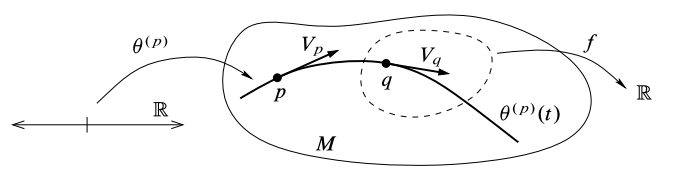
\includegraphics[scale = 0.42]{infinitesimal_generator_flow.png}}
\end{minipage}
\caption{\footnotesize{\textbf{The infinitesimal generator of the globla flow  \citep{lee2003introduction}}}}
\label{fig: infinitesimal_generator_flow}
\end{figure}

\item \begin{definition}
If $\theta: \bR \times M \rightarrow M$ is a smooth global flow, for each $p \in M$ we define a \emph{tangent vector $V_p \in T_pM$} by
\begin{align*}
V_p &=  (\theta^{(p)})'(0) = d\theta^{(p)}\paren{\frac{d}{dt}\Bigr|_{t=0}}.
\end{align*} 
The assignment $p \mapsto V_p$ is \emph{\textbf{a (rough) vector field}} on $M$; which is called \emph{\textbf{the infinitesimal generator of the global flow $\theta$}}.
\end{definition}

\begin{remark}
$V$ is the \emph{infinitesimal generator} of the flow $\theta$ $\Leftrightarrow$ $\theta$ is the \emph{integral curve} of $V$.
\end{remark}

\item \begin{proposition}
Let $\theta: \bR \times M \rightarrow M$ be a smooth global flow on a smooth manifold $M$. The infinitesimal generator $V$ of $\theta$ is a smooth vector field on $M$; and each curve $\theta^{(p)}$ is \textbf{an integral curve} of $V$.
\end{proposition} This means that $(\theta^{(p)})'(t) = V_{\theta^{(p)}(t)}$ for all $p \in M$ and all $t \in \bR$.
\end{itemize}


\subsection{The Fundamental Theorem on Flows}

\begin{itemize}
\item We have seen that \textbf{\emph{every smooth global flow}} gives rise to \textbf{\emph{a smooth vector field}} whose \textbf{\emph{integral curves}} are precisely \emph{the curves defined by the flow}. 

Conversely, however, it is \textbf{not true} that every smooth vector field is the infinitesimal generator of a smooth global flow.

\item \begin{definition}
If $M$ is a manifold, a \emph{\textbf{flow domain}} for $M$ is an open subset $\mathfrak{D} \subseteq \bR \times M$ with the property that for each $p \in M$,
the set $\mathfrak{D}^{(p)} = \set{t \in \bR: (t, p) \in \mathfrak{D}}$ is an \emph{open interval} \emph{\textbf{containing}} $0$ (Fig. \ref{fig: flow_domain}).

A \underline{\emph{\textbf{flow}}} on $M$ is a continuous map $\theta: \mathfrak{D} \rightarrow M$; where  $\mathfrak{D} \subseteq \bR \times M$ is \emph{a flow domain}, that satisfies the following \emph{\textbf{group laws}}: 
\begin{align}
\theta(0, p) &=p, \quad \forall p \in M  \label{eqn: local_flow_group_identity}\\
\theta(t, \theta(s, p)) &= \theta(t+s, p), \quad \forall s \in \mathfrak{D}^{(p)}, \; t \in \mathfrak{D}^{(\theta(s, p))},\; (\text{i.e. }t+s \in \mathfrak{D}^{(p)})  \label{eqn: local_flow_group}
\end{align} We sometimes call $\theta$ \underline{\emph{\textbf{a local flow}}} to distinguish it from \emph{a global flow} as defined earlier. The unwieldy term \emph{\textbf{local one-parameter group action}} is also used.
\end{definition}

\begin{figure}
\begin{minipage}[hb]{1\linewidth}
  \centering
  \centerline{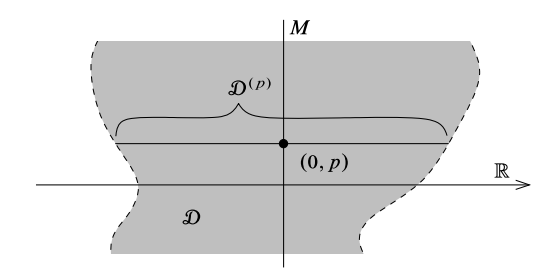
\includegraphics[scale = 0.42]{flow_domain.png}}
\end{minipage}
\caption{\footnotesize{\textbf{The flow domain  \citep{lee2003introduction}}}}
\label{fig: flow_domain}
\end{figure}

\item \begin{definition}
If $\theta$ is a flow, we define $\theta_t(p) = \theta^{(p)}(t) = \theta(t, p)$ whenever $(t, p) \in \mathfrak{D}$, just as for a global flow. For each $t \in \bR$, we also define
\begin{align}
M_t = \set{p \in M: (t, p) \in \mathfrak{D}} \label{eqn: local_flow_starting_points}
\end{align} so that
\begin{align*}
p \in M_t \Leftrightarrow t \in \mathfrak{D}^{(p)} \Leftrightarrow (t,p) \in \mathfrak{D}.
\end{align*} If $\theta$ is smooth, \emph{\textbf{the infinitesimal generator}} of $\theta$ is defined by $V_p =  (\theta^{(p)})'(0)$.
\end{definition}

\item \begin{proposition}
If $\theta: \mathfrak{D} \rightarrow M$ is a smooth flow, then the infinitesimal generator $V$ of $\theta$ is a smooth vector field, and each curve $\theta^{(p)}$ is an integral curve of $V$.
\end{proposition}

\item \begin{definition}
\emph{A \textbf{maximal integral curve}} is one that cannot be extended to an integral curve on \emph{any larger open interval}, and \emph{a \textbf{maximal flow}} is a flow that admits \emph{no extension} to a flow on a \emph{larger flow domain}.
\end{definition}

\item \begin{theorem} (\textbf{Fundamental Theorem on Flows}). \citep{lee2003introduction}\\
Let $V$ be a smooth vector field on a smooth manifold $M$. There is a \textbf{unique smooth maximal flow} $\theta: \mathfrak{D} \rightarrow M$
whose \textbf{infinitesimal generator} is $V$. This flow has the following properties:
\begin{enumerate}
\item For each $p \in M$, the curve $\theta^{(p)}: \mathfrak{D}^{(p)} \rightarrow M$ is the \textbf{unique maximal integral curve} of $V$ starting at $p$.
\item If $s \in \mathfrak{D}^{(p)}$, then $\mathfrak{D}^{(\theta(s, p))}$ is the interval $\mathfrak{D}^{(p)} - s = \set{t - s: t \in \mathfrak{D}^{(p)}}$.
\item For each $t \in \bR$, the set $M_t$ is \textbf{open} in $M$; and $\theta_t: M_t \rightarrow M_{-t}$ is a \textbf{diffeomorphism} with \textbf{inverse} $\theta_{-t}$.
\end{enumerate}
\end{theorem}

\item \begin{remark}
The flow whose \emph{\textbf{existence}} and \emph{\textbf{uniqueness}} are asserted in the fundamental theorem is called \emph{\textbf{the flow generated by $V$}} , or just \underline{\emph{\textbf{the flow of $V$}}}. 
\end{remark}


\item \begin{proposition} (\textbf{Naturality of Flows}). \citep{lee2003introduction} \\
Suppose $M$ and $N$ are smooth manifolds, $F: M \rightarrow N$ is a smooth map,  $X \in \mathfrak{X}(M)$, and $Y \in \mathfrak{X}(N)$.  Let $\theta$ be the flow of $X$
and $\eta$ the flow of $Y$. If $X$ and $Y$ are $F$-related, then for each $t \in \bR$, $F(M_t) \subseteq N_t$ and $\eta_t \circ F = F \circ \theta_t$ on $M_t$:
\[
  \begin{tikzcd}
    M_t \arrow{r}{F} \arrow[swap]{d}{\theta_t} & N_t \arrow{d}{\eta_t} \\
    M_{-t} \arrow{r}{F} & N_{-t}
  \end{tikzcd}
\]
\end{proposition}

\item \begin{corollary} (\textbf{Diffeomorphism Invariance of Flows}).\\
 Let $F: M \rightarrow N$ be a diffeomorphism. If $X \in \mathfrak{X}(M)$ and $\theta$ is the flow of $X$, then the \textbf{flow of pushforward} $F_{*}X$ is $\eta_t =   F \circ \theta_t \circ F^{-1}$, with domain $N_t = F(M_t)$ for each $t \in \bR$. 
\end{corollary}
\end{itemize}


\subsection{Complete Vector Fields}
\begin{itemize}
\item As we observed earlier in this chapter, not every smooth vector field generates a \emph{global flow}. The ones that do are important enough to deserve a name. 
\begin{definition}
We say that\emph{ a smooth vector field} is \emph{\textbf{complete}} if it generates a \emph{\textbf{global flow}}, or equivalently if \emph{each} of its \emph{maximal integral curves} is defined for \emph{\textbf{all} $t \in \bR$}. 
\end{definition}

\item We will show below that \emph{all compactly supported smooth vector fields, and therefore all smooth vector fields on a compact manifold, are complete}. The proof will
be based on the following lemma.

 \begin{lemma} (\textbf{Uniform Time Lemma}).\\
 Let $V$ be a smooth vector field on a smooth manifold $M$, and let $\theta$ be its flow. Suppose there is \textbf{a positive number} $\epsilon$ such that for
\textbf{every} $p \in M$, the domain of $\theta^{(p)}$ contains $(-\epsilon, \epsilon)$. Then $V$ is complete.
\end{lemma}

\item \begin{theorem}
Every \textbf{compactly supported} smooth vector field on a smooth manifold is \textbf{complete}.
\end{theorem}

\item \begin{corollary} 
On a \textbf{compact smooth manifold}, \textbf{every} smooth vector field is \textbf{complete}. 
\end{corollary}

\item \emph{Left-invariant vector fields on Lie groups} form another class of vector fields that are always complete.
\begin{theorem}
Every \textbf{left-invariant} vector field on a \textbf{Lie group} is complete.
\end{theorem}

\item Here is another useful property of integral curves.
\begin{lemma}  (\textbf{Escape Lemma}).\\
Suppose $M$ is a smooth manifold and $V \in \mathfrak{X}(M)$. If $\gamma:  J \rightarrow M$ is a maximal integral curve of $V$ whose domain $J$ has a finite least
upper bound $b$, then for any $t_0 \in J$, $\gamma([t_0, b))$ is not contained in \textbf{any compact subset} of $M$.
\end{lemma}
\end{itemize}





\section{Flowouts}
\begin{itemize}
\item 
\end{itemize}

\section{Flows and Flowouts on Manifolds with Boundary}


\section{Lie Derivatives}
\begin{figure}
\begin{minipage}[hb]{1\linewidth}
  \centering
  \centerline{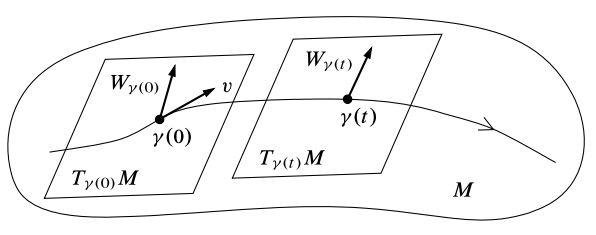
\includegraphics[scale = 0.42]{directional_derivative_of_vector_fields.png}}
\end{minipage}
\caption{\footnotesize{\textbf{The directional derivative of vector fields  \citep{lee2003introduction}}}}
\label{fig: directional_derivative_of_vector_fields}
\end{figure}
\begin{itemize}
\item The directional derivatives of a smooth function on $M$ is obtained via $vf$ where $v$ is a tangent vector operator $v\in T_pM$. What about the directional derivative of a vector field? 

\item \begin{remark}
In \emph{Euclidean space}, it makes sense to ask this question. We can define \emph{the directional derivatives of a vector field $W$ at point $p$} as below:
\begin{align*}
D_{v}W(p) &:=   \lim_{t\rightarrow 0} \frac{W_{p+ t\,v} - W_{p}}{t} = \frac{d}{dt}\Bigr|_{t=0}W_{p+t\,v}.
\end{align*} An easy calculation shows that $D_{v}W(p)$ can be evaluated by applying $D_v$ to each component of $W$ separately (See Fig \ref{fig: directional_derivative_of_vector_fields}.):
\begin{align*}
D_{v}W(p) &= D_{v}W^{i}(p)\,\partdiff{}{x^{i}}\Bigr|_{p}.
\end{align*} 

\emph{Unfortunately}, this definition is heavily dependent upon the fact that $\bR^n$ is a \emph{\textbf{vector space}}, so that \emph{the tangent vectors $W_{p+tv}$ and $W_p$ can \textbf{both} be viewed as elements} of $\bR^{n}$.
\end{remark}

\item \begin{remark}
For a manifold $M$, the vector field $W_{p+tv}$ may not be well-defined since we do not know if $p+tv \in M$. Therefore, we replace $p + tv$ by the curve $\gamma(t)=\theta(p, t)$ where $\gamma(0) = p$ and $\gamma'(0) = v$. On the other hand, the vector field $W_{\gamma(0)}$ and $W_{\gamma(t)}$ are \emph{not in the same tangent space} (one in $T_{\gamma(0)}M$ and the other $T_{\gamma(t)}M$).  We got away with it in Euclidean space because there is a canonical identification
of each tangent space with $\bR^n$ itself; this is not true for general smooth manifold $M$.

This problem can be circumvented if we replace the vector $v \in T_{p}M$ with a \emph{\textbf{vector field}} $V \in \mathfrak{X}(M)$, so we can use the \emph{\textbf{flow}} of $V$ to \emph{\textbf{push values of $W$ back to $p$}} and then differentiate.
\end{remark}


\item \begin{definition}
Suppose $M$ is a smooth manifold, $V$ is a \emph{smooth vector field} on $M$; and $\theta$ is the \emph{\textbf{flow of $V$}}. For any
smooth vector field $W$ on $M$, define \emph{\textbf{a rough vector field}} on $M$, \emph{denoted by} $\mathscr{L}_{V}\,W$ and called the \underline{\emph{\textbf{Lie derivative} of $W$ with respect to $V$}}, by
\begin{align}
\paren{\mathscr{L}_{V}\,W}_{p} &= \lim_{t\rightarrow 0}\frac{ d(\theta_{-t})_{\theta_{t}(p)}\paren{W_{\theta_t(p)}}   - W_{p}}{t} \label{eqn: lie_derivative_formula}\\
&= \frac{d}{dt}\Bigr|_{t=0} d\paren{\theta_{-t}}_{\theta_{t}(p)}\paren{W_{\theta_t(p)}}  \nonumber,
\end{align}
provided the derivative exists. For small $t \neq 0$, at least the difference quotient makes sense: $\theta_t$ is defined in a neighborhood of $p$, and $\theta_{-t}$ is the inverse of $\theta_t$, so both $d(\theta_{-t})_{\theta_{t}(p)}\paren{W_{\theta_t(p)}}$ and $W_p$ are elements of $T_{p}M$ (Fig \ref{fig: lie_derivatives}).
\end{definition}

\begin{figure}
\begin{minipage}[hb]{1\linewidth}
  \centering
  \centerline{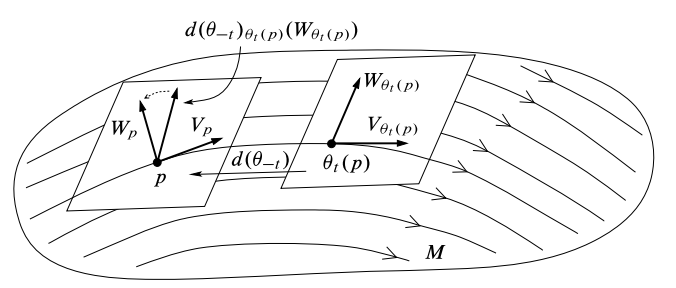
\includegraphics[scale = 0.42]{lie_derivatives.png}}
\end{minipage}
\caption{\footnotesize{\textbf{The Lie derivative of vector fields  \citep{lee2003introduction}}}}
\label{fig: lie_derivatives}
\end{figure}

\item \begin{remark}
If $M$ has nonempty boundary, this definition of  $\mathscr{L}_{V}\,W$ makes sense as long as $V$ is tangent to $\partial M$ so that its flow exists.
\end{remark}

\item \begin{lemma}
Suppose $M$ is a smooth manifold with or without boundary, and $V, W \in \mathfrak{X}(M)$. If $\partial M \neq \emptyset$, assume in addition that $V$ is tangent to $\partial M$. Then $(\mathscr{L}_{V}\,W)_{p}$ exists for every $p \in M$, and $\mathscr{L}_{V} W$ is a \textbf{smooth vector field}.
\end{lemma}
\begin{proof}
Let $\theta$ be the flow of $V$. For arbitrary $p\in M$, let $(U, (x^i))$ be a smooth chart containing $p$. Choose an open interval $J_0$ containing $0$ and an open subset $U_0 \subseteq U$ containing $p$ such that $\theta$ maps $J_0 \times U_0$ into $U$. For $(t, x) \in J_0 \times U_0$, write the component functions of $\theta$ as $(\theta^1(t, x), \ldots, \theta^{n}(t, x))$. Then for any $(t, x)\in J_0 \times U_0$, the matrix of $d(\theta_{-t})_{\theta_t(x)}: T_{\theta_t(x)}M \rightarrow T_{x}M$ is
\begin{align*}
\paren{\partdiff{\theta^{i}}{x^{j}}(-t,  \theta(t, x))}.
\end{align*}
Therefore,
\begin{align*}
d\paren{\theta_{-t}}_{\theta_{t}(p)}\paren{W_{\theta_t(p)}} &= \partdiff{\theta^{i}}{x^{j}}(-t,  \theta(t, x)) W^{j}(\theta(t, x))\,\partdiff{}{x^{i}}\Bigr|_{x}.
\end{align*}
Because $\theta^i$ and $W^j$ are smooth functions, the coefficient of $\partial / \partial x^i |_{x}$ depends smoothly on $(t, x)$. It follows that $(\mathscr{L}_{V}\,W)_{x}$, which is obtained by taking the derivative of this expression with respect to $t$ and setting $t = 0$, exists for each $x \in U_0$ and depends smoothly on $x$.  \qed
\end{proof}

\item The following theorem is critical to understand the \emph{\textbf{Lie derivatives}} and \emph{\textbf{Lie bracket}}.
\begin{theorem}
If $M$ is a smooth manifold and $V, W \in \mathfrak{X}(M)$, then $\mathscr{L}_{V}\,W = [V, W]$.
\end{theorem}
\begin{proof}
Suppose $V, W \in \mathfrak{X}(M)$, and let $\cR(V) \subseteq M$ be the set of \emph{regular points} of $V$ (the set of points $p \in M$ such that $V_p \neq 0$). Note that $\cR(V)$ is \emph{open} in $M$ by continuity, and its \emph{closure} is the support of $V$. We will show that $(\mathscr{L}_{V}\,W)_{p} = [V, W]_p$ for all $p \in M$, by considering three cases.
\begin{itemize}
\item $p \in \cR(V)$. In this case, we can choose smooth coordinates $(u^i)$ on a neighborhood of $p$ in which $V$ has the coordinate representation $V = \partial/\partial u^{1}$ (Theorem 9.22). In these coordinates, the \emph{flow} of $V$ is $\theta_t(u) = (u^1+ t,u^2,\ldots,u^n)$. For each fixed $t$, the matrix of $d(\theta_{-t})_{\theta_t(x)}$ in these coordinates (\emph{the Jacobian matrix} of $\theta_{-t}$) is the \emph{identity at every point}. Consequently, for any $u \in U$,
\begin{align*}
d\paren{\theta_{-t}}_{\theta_{t}(u)}\paren{W_{\theta_t(u)}} &= d\paren{\theta_{-t}}_{\theta_{t}(u)}\paren{W^{j}(u^1+ t, u^2, \ldots, u^n)\,\partdiff{}{u^{j}}\Bigr|_{\theta_t(u)}}\\
&= W^{j}(u^1+ t, u^2, \ldots, u^n)\,\partdiff{}{u^{j}}\Bigr|_{u}.
\end{align*} Using the definition of the Lie derivative, we obtain
\begin{align*}
\paren{\mathscr{L}_{V}\,W}_{u} &= \frac{d}{dt}\Bigr|_{t=0} W^{j}(u^1+ t, u^2, \ldots, u^n)\,\partdiff{}{u^{j}}\Bigr|_{u} = \partdiff{W^{j}}{u^1}(u^1, u^2, \ldots, u^n)\,\partdiff{}{u^{j}}\Bigr|_{u}.
\end{align*} On the other hand, by virtue of formula (note that $V_i =0$ for all $i\neq 1$ and $V_1 = 1$.)
\begin{align}
[V, W]&= \paren{V^{i}\,\partdiff{W^{j}}{u^{i}} - W^{i}\,\partdiff{V^{j}}{u^{i}} }\partdiff{}{u^{j}} \label{eqn: lie_bracket}\\
&= \paren{\partdiff{W^{j}}{u^{1}} }\partdiff{}{u^{j}},  \nonumber
\end{align}
 for the Lie bracket in coordinates, $[V, W]_u$ is easily seen to be equal to the same expression.
 
\item $p \in \text{supp}(V)$. Because $\text{supp}V$ is the closure of $\cR(V)$, it follows by continuity from Case 1 that $(\mathscr{L}_{V}\,W)_{p} = [V, W]_p$  for $p \in \text{supp}(V)$.

\item $p \in M \setminus \text{supp}(V)$. In this case, $V\equiv 0$ on a neighborhood of $p$. On the one hand, this implies that $\theta_t$ is equal to the identity map in a neighborhood of $p$ for all $t$, so $d\paren{\theta_{-t}}_{\theta_{t}(p)}\paren{W_{\theta_t(p)}} = W_p$, which implies  $(\mathscr{L}_{V}\,W)_{p} = 0$. On the other
hand, $[V, W]_p =0$ by formula \eqref{eqn: lie_bracket}. \qed
\end{itemize}
\end{proof}



\item \begin{remark}
This theorem allows us to extend the definition of the \emph{\textbf{Lie derivative}} to arbitrary \emph{smooth vector fields} on a smooth manifold $M$ with boundary. Given $V, W \in \mathfrak{X}(M)$ we define $(\mathscr{L}_{V}\,W)_{p}$ for $p \in \partial M$ by embedding $M$ in a smooth manifold $\widetilde{M}$ without boundary (such as the double of $M$), extending $V$ and $W$ to smooth vector fields on $\widetilde{M}$, and computing the Lie derivative there. By virtue of the preceding theorem,
$(\mathscr{L}_{V}\,W)_{p} = [V, W]_p$ is independent of the choice of extension.
\end{remark}

\item \begin{remark} This thoerem also gives us a \emph{\textbf{geometric interpretation}} of \emph{the Lie bracket of two vector fields}: it is the \emph{\textbf{directional derivative} of the second vector field} along \emph{the \textbf{flow} of the first}. 
\end{remark}

\item \begin{corollary}
Suppose $M$ is a smooth manifold with or without boundary, and $V, W, X \in \mathfrak{X}(M)$.
\begin{enumerate}
\item (\textbf{Anti-symmetric}) $\mathscr{L}_{V}\,W = -\mathscr{L}_{W}\,V$.
\item $\mathscr{L}_{V}\,[W,\, X] =  [\mathscr{L}_{V}\,W, \,X] + [W,\, \mathscr{L}_{V}\,X]$.
\item (\textbf{Lie Bracket definition}) $\mathscr{L}_{[V, W]}\,X = \mathscr{L}_{V}\mathscr{L}_{W}\,X - \mathscr{L}_{W}\mathscr{L}_{V}\,X$.
\item If $g \in \cC^{\infty}(M)$, then $\mathscr{L}_{V}\,(gW) = (Vg)\,W + g\,\mathscr{L}_{V}\,W$.
\item (\textbf{Pushforward}) If $F: M \rightarrow N$ is a \textbf{diffeomorphism}, then $F_{*}(\mathscr{L}_{V}\,X) = \mathscr{L}_{F_{*}V}\,F_{*}X$.
\end{enumerate}
\end{corollary}

\item \begin{remark}
Note that the Lie derivative is \emph{\textbf{not linear over $\cC^{\infty}(M)$ in $V$}}, i.e.
\begin{align*}
\mathscr{L}_{fV}\,W &\neq f\,\mathscr{L}_{V}\,W
\end{align*}
\end{remark}

\item \begin{remark}
If $V$ and $W$ are vector fields on $M$ and $\theta$ is the flow of $V$, the Lie derivative $(\mathscr{L}_{V}\,W)_{p}$, by definition, expresses the $t$-derivative of \emph{the \textbf{time-dependent vector}} $d\paren{\theta_{-t}}_{\theta_{t}(p)}\paren{W_{\theta_t(p)}}  \in T_{p}M$ at $t = 0$. The next proposition shows how it can also
be used to compute the derivative of this expression at other times. 
\end{remark}

\item \begin{proposition}
Suppose $M$ is a smooth manifold with or without boundary and $V, W \in \mathfrak{X}(M)$. If $\partial M \neq \emptyset$, assume also that $V$ is tangent to $\partial M$. Let $\theta$ be the flow of $V$. For any $(t_0, p)$ in the domain of $\theta$,
\begin{align}
 \frac{d}{dt}\Bigr|_{t=t_0} d\paren{\theta_{-t}}_{\theta_{t}(p)}\paren{W_{\theta_t(p)}}&= d(\theta_{-t_0})\paren{(\mathscr{L}_{V}\,W)_{\theta_{t_0}(p)}}.  \label{eqn: lie_derivative_at_other_time}
\end{align}
\end{proposition}

\end{itemize}



\section{Commuting Vector Fields}
\subsection{Commuting Vector Fields}
\begin{itemize}
\item \begin{definition}
Let $M$ be a smooth manifold and $V, W \in \mathfrak{X}(M)$. We say that $V$ and $W$ \underline{\emph{\textbf{commute}}} if $VW\,f = WV\,f$ for every smooth function $f$, or equivalently if $[V, W] \equiv 0$. 
\end{definition}

\item \begin{definition}
If $\theta: \mathfrak{D} \rightarrow M$ is a \emph{\textbf{smooth flow}}, a vector field $W$ is said to be \emph{\textbf{\underline{invariant} under $\theta$}} if $W$ is \emph{\textbf{$\theta_t$-related to itself}} for each $t$; more precisely, this means that $W|_{M_t}$ is $\theta_t$ -related to $W|_{M_{-t}}$ for each $t$, or equivalently that 
\begin{align*}
d(\theta_{t})_{p}(W_p) &= W_{\theta_t(p)}, \quad \forall\,(t,p) \in \mathfrak{D}
\end{align*}
\end{definition}

\item \begin{theorem}
For smooth vector fields $V$ and $W$ on a smooth manifold $M$,  the following are equivalent:
\begin{enumerate}
\item $V$ and $W$ \textbf{commute}.
\item $W$ is \textbf{invariant} under the \textbf{flow} of $V$.
\item $V$ is \textbf{invariant} under the \textbf{flow} of $W$.
\end{enumerate}
\end{theorem}

\item \begin{corollary}
Every smooth vector field is invariant under its own flow.
\end{corollary} Note that $[V, V] \equiv 0$.

\item \begin{definition}
If $\theta$ and $\psi$ are flows on $M$, we say that $\theta$ and $\psi$ \emph{\textbf{commute}} if the following condition holds for every $p \in M$: 
whenever $J$ and $K$ are open intervals containing $0$ such that \emph{one of the expressions} $\theta_t \circ \psi_s(p)$ or $\psi_s  \circ \theta_t (p)$ is defined for \emph{\textbf{all}} $(s, t) \in J \times K$, \emph{\textbf{both are defined}} and \textbf{\emph{they are equal}}.

For global flows, this is the same as saying that $\theta_t \circ \psi_s = \psi_s  \circ \theta_t$ for all $s$ and $t$.
\end{definition}

\item 
\begin{theorem}
\textbf{Smooth vector fields commute} if and only if \textbf{their flows commute}.
\end{theorem}
\end{itemize}

\subsection{Commuting Frames}

\section{Time-Dependent Vector Fields}

%\section{First-Order Partial Differential Equations}


\newpage
\bibliographystyle{plainnat}
\bibliography{book_reference.bib}
\end{document}